\section{Introduction}
\label{sec:introduction}

When multiple LLM judges evaluate model responses on a benchmark, their scores are shaped by at least three forces: the model's genuine ability, the judge's own scoring tendency, and any advantage the model gained from encountering benchmark items during training. These three signals are entangled in every observation. The evaluation community has developed separate tools for the latter two distortions: judge bias correction methods calibrate inter-judge differences \citep{cyclicjudge2026, uda2026}, while contamination detection tools flag or adjust for memorized items \citep{constat2024, dcr2025, logprober2024}. A practitioner who faces both problems must apply these corrections sequentially. This paper shows that sequential correction produces systematically biased rankings, not merely noisy ones.

\begin{figure*}[t]
\centering
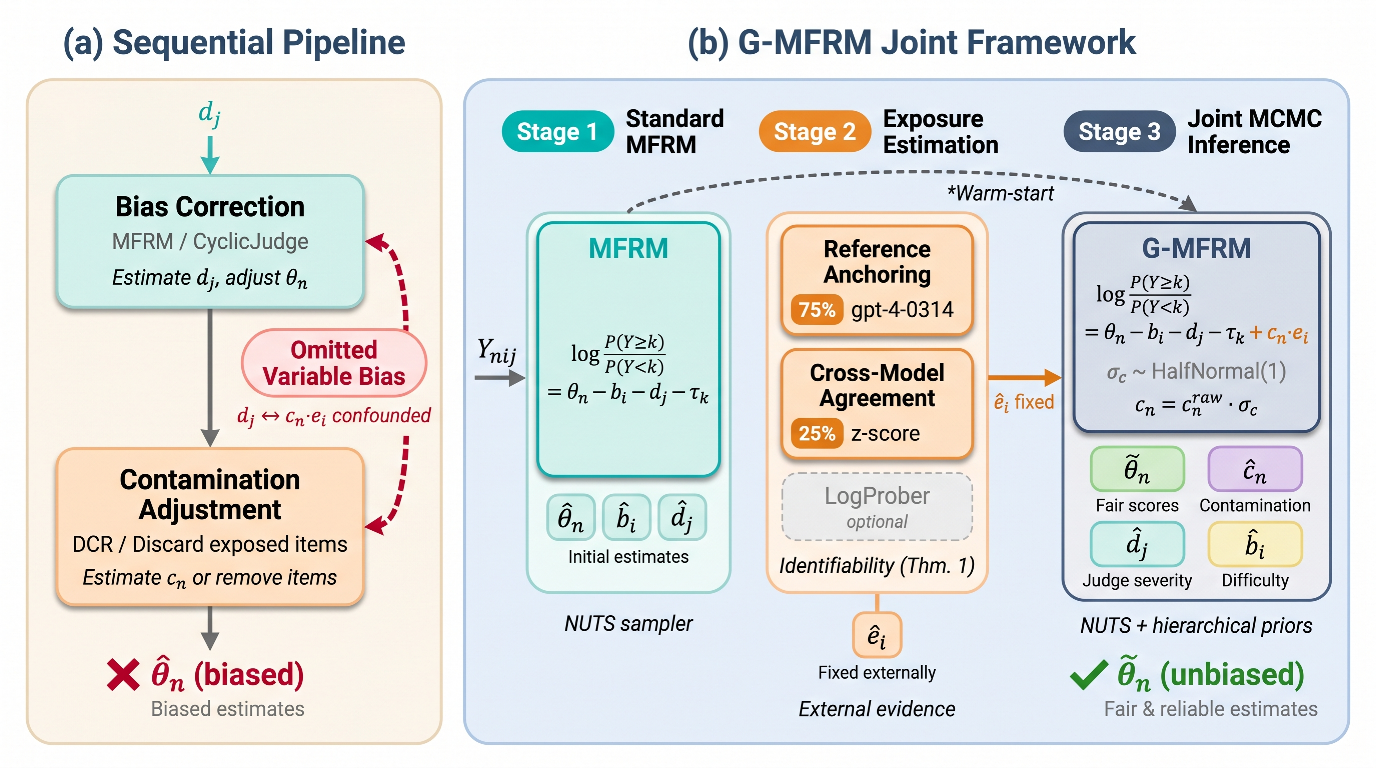
\includegraphics[width=\textwidth]{fig1_framework_v2}
\caption{(a)~Sequential pipelines address judge bias and contamination independently; omitted variable bias confounds the unmodeled facet into ability estimates. (b)~G-MFRM three-stage joint calibration: Stage~1 fits a standard MFRM for initial estimates $(\hat{\theta}, \hat{b}, \hat{d})$; Stage~2 estimates per-item exposure $e_i$ from external evidence (reference model anchoring, cross-model agreement, and optionally LogProber); Stage~3 performs joint MCMC inference with $e_i$ fixed, recovering contamination-corrected ability $\hat{\theta}_n$, contamination susceptibility $c_n$, and judge severity $d_j$.}
\label{fig:framework}
\end{figure*}

We formalize this failure as an omitted variable bias (OVB) problem \citep{angrist2009mostly}. Consider a model that has memorized some benchmark items and a judge that scores more strictly than average. A bias-only correction adjusts for the strict judge but leaves the contamination signal untouched; the inflated scores on memorized items get absorbed into the model's estimated ability. Conversely, a contamination-only adjustment removes the memorization signal but conflates systematic scoring differences with contamination variation. In both cases, the omitted facet biases the modeled one. Within the Many-Facet Rasch Model (MFRM) framework \citep{linacre1989mfrm}, we show this bias is directional: contaminated models are systematically overestimated under bias-only correction, and the bias persists regardless of which correction comes first (Section~\ref{sec:confounding}).

Resolving this confounding requires joint estimation. We propose the Gated Many-Facet Rasch Model (G-MFRM), which extends MFRM with a multiplicative gating term $c_n \cdot e_i$ for contamination susceptibility, inspired by Doubly-Gated Item Response Theory \citep{shu2013dgirt}. Through a three-stage calibration procedure with externally anchored per-item exposure indicators (Figure~\ref{fig:framework}), G-MFRM simultaneously recovers model ability, item difficulty, judge severity, and contamination susceptibility. We prove that external anchoring of exposure is both necessary and sufficient for parameter identification under standard multi-judge designs (Theorem~\ref{thm:sufficient}), and derive error propagation bounds for the staged estimation.

In synthetic experiments ($N = 50$ models, 20 seeds), G-MFRM reduces ability RMSE by 51\% relative to sequential estimation ($p < 0.001$) and recovers contamination susceptibility with Pearson $r = 0.81$. On Arena-Hard \citep{li2024arenahard}, G-MFRM produces interpretable per-model contamination diagnostics (in an 8-model pilot, older models such as GPT-3.5-Turbo and GPT-4-0613 exhibit 4--6$\times$ higher susceptibility than recent models such as GPT-4o), and a controlled coverage ablation with 17 models and 6 judges traces over-correction to incomplete exposure estimation ($\Delta\tau$: $-0.044 \to -0.015 \to 0.000$ as coverage increases from 46\% to 100\%). Leave-one-out cross-validation strongly favors joint estimation (expected log pointwise predictive density difference $|\Delta\mathrm{ELPD}/\mathrm{SE}| = 5.9$; stacking weight 1.0). Our contributions are:
\begin{enumerate}
    \item A formal analysis of judge-contamination confounding as omitted variable bias, proving that sequential correction cannot resolve the confounding under non-orthogonality (Section~\ref{sec:confounding}).
    \item The G-MFRM framework with identifiability guarantees and error propagation bounds for staged estimation (Section~\ref{sec:method}).
    \item Empirical validation on Arena-Hard yielding interpretable contamination diagnostics, with a controlled coverage ablation tracing over-correction to incomplete exposure estimation (Section~\ref{sec:experiments}).
\end{enumerate}
